\lhead{\emph{Datasets}}
\chapter{Datasets} \label{datasets}

All quality measures described in Chapter \ref{quality_measures} obtained and presented in this paper are calculated from classifiers' results for certain datasets. Those sets, referred to as native and foreign, are the result of applying feature-extraction function to images containing digits and letters. The original data comes from the well-known MNIST database\cite{MNIST}, which comprises the image files of handwritten upper-case letters, which have been size-normalized and centered in a fixed-size image. It is a good database for people who want to try learning techniques and pattern recognition methods on real-world data while spending minimal efforts on preprocessing and formatting.

\begin{figure}[htp]
	\centering
	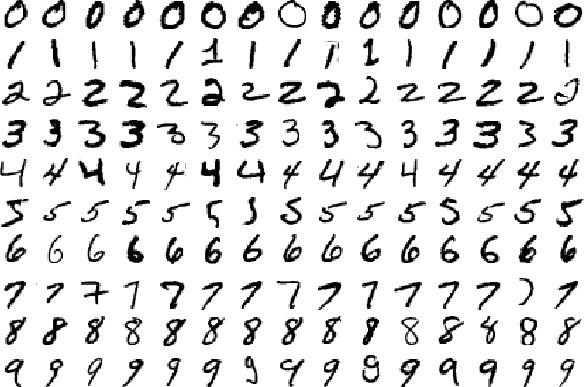
\includegraphics[width=0.7\textwidth]{Figures/mnistdigits.jpg}
	\caption{Visualization of scanned digits from MNIST database, image taken from \cite{Kuan_Hoong_Blog}}
	\label{fig:mnist_digits}\vspace{-3pt}
\end{figure}

The native set consists of 10,000 scanned digit images, with ten different classes one for every digit (0 - 9) and approximately 1000 samples for each class. This set is further divided into training and test sets in 7:3 ratio. The foreign set consists of 26,000 images of scanned letters and is not divided internally because it is used only in rejection option evaluation. All patterns within those two sets have been size-normalized and centred in a fixed-size image. Every pattern within those two datasets consists of 24 unique features that were extracted to ensure best classification capabilities. Examples of features are: maximum/position of maximum values of projections, histograms of projections, transitions, offsets; raw moments, central moments, Euler numbers etc. 